%!TEX root = slide.tex

\section{Subprogramas Como Parâmetro}
\begin{frame}{Subprogramas Como Parâmetro}
	\begin{itemize}
	  \item Ideia simples, mas gera complicações.
	  \item \emph{Type checking}.
	  \item referencing environment.
	\end{itemize}
\end{frame}

\begin{frame}{Referencing Environment}
	\begin{itemize}
	  \item Linguagens que permitem subprogramas aninhados.
	  \item Shallow Binding
	  \item Deep Binding
	  \item Ad Hoc Binding
	\end{itemize}
\end{frame}

\begin{frame}{Exemplo}
	\begin{figure}[ht!]
		\centering
		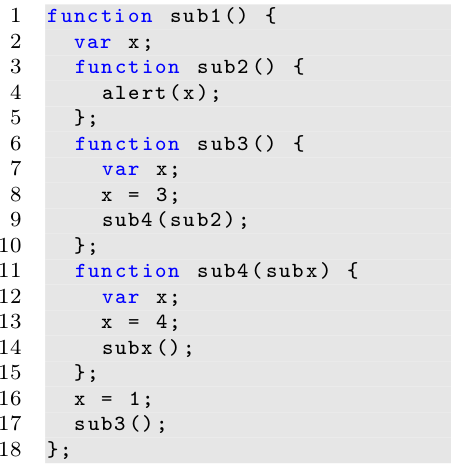
\includegraphics[scale=0.4]{./imgs/js-original}
	\end{figure}
\end{frame}

\begin{frame}{Shallow Binding}
	O ambiente é o local onde o subprograma é chamado.
\end{frame}

\begin{frame}{Shallow Binding}
	\begin{figure}[ht!]
		\centering
		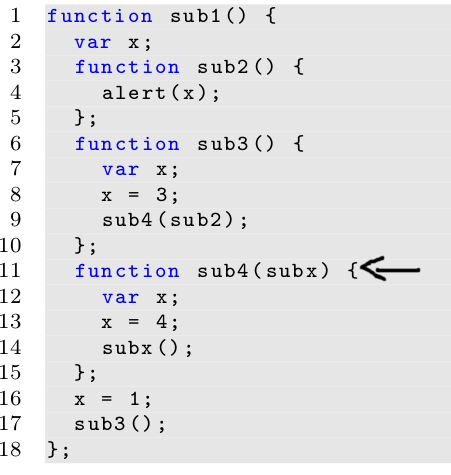
\includegraphics[scale=0.4]{./imgs/js-shallow}
	\end{figure}
\end{frame}

\begin{frame}{Deep Binding}
	O ambiente refere-se onde o subprograma foi definido.
\end{frame}

\begin{frame}{Deep Binding}
	\begin{figure}[ht!]
		\centering
		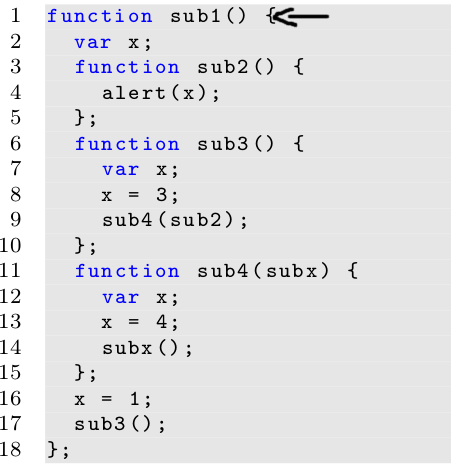
\includegraphics[scale=0.4]{./imgs/js-deep}
	\end{figure}
\end{frame}

\begin{frame}{Ad Hoc Binding}
	O ambiente condiz com o local que o subprograma foi passado por parâmetro.
	Nunca implementado.
\end{frame}

\begin{frame}{Ad Hoc Binding}
	\begin{figure}[ht!]
		\centering
		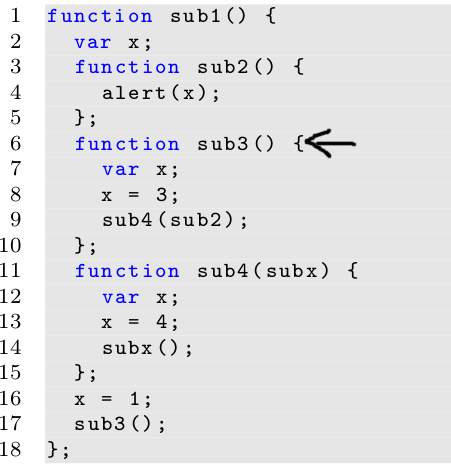
\includegraphics[scale=0.4]{./imgs/js-adhoc}
	\end{figure}
\end{frame}

\section{Chamar Subprogramas Indiretamente}
\begin{frame}{Chamar Subprogramas Indiretamente}
	\begin{itemize}
	  \item Subprograma conhecido em tempo de execução.
	  \item GUI e callback.
	  \item C/C++ ponteiro para função.
	  \item C\# Delegate.
	\end{itemize}
\end{frame}

\begin{frame}[fragile]{C/C++ - Ponteiro Para Função}
	\begin{lstlisting}[language=c]
		//declaracao da funcao
		int sum(int a, int b)
		{
			return a + b;
		}

		//ponteiro para a funcao
		int (*sum_pointer)(int, int);
		sum_pointer = &sum;
		
		//chamar a funcao
		(*sum_pointer)(1,2);
	\end{lstlisting}
\end{frame}

\begin{frame}[fragile]{C\# - Delegate}
	\begin{lstlisting}[language=csh]
		//declarar um delegate
		public delegate int SumDelegate(int a, int b);
		...
		//instanciar um delegate (funcao sum tem a mesma assinatura)
		SumDelegate sumDelegate = new SumDelegate(sum);
		//executar
		sumDelegate(2,3);
	\end{lstlisting}
\end{frame}